% ============================================
% ===== CAPÍTULO 3: PLANIFICACIÓN =====
% ============================================
\chapter{Planificación}\label{chap:planificacion}
Una vez definidos los requisitos y la metodología a seguir, el siguiente paso es planificar de forma concreta el proyecto. En esta fase se crearán los distintos módulos del proyecto (EDT), se establecerán las fechas límite para los entregables y se estimará el tiempo necesario para cada apartado. Además, se incluirá un cronograma de hitos y un diagrama del flujo de trabajo. Posteriormente, se diseñará un plan de gestión de riesgos basándose en la metodología aprendida durante la carrera. El capítulo concluye con la descripción de las tecnologías utilizadas.

\section{Descomposición del Proyecto (EDT)}
\begin{figure}[h!]
    \centering
    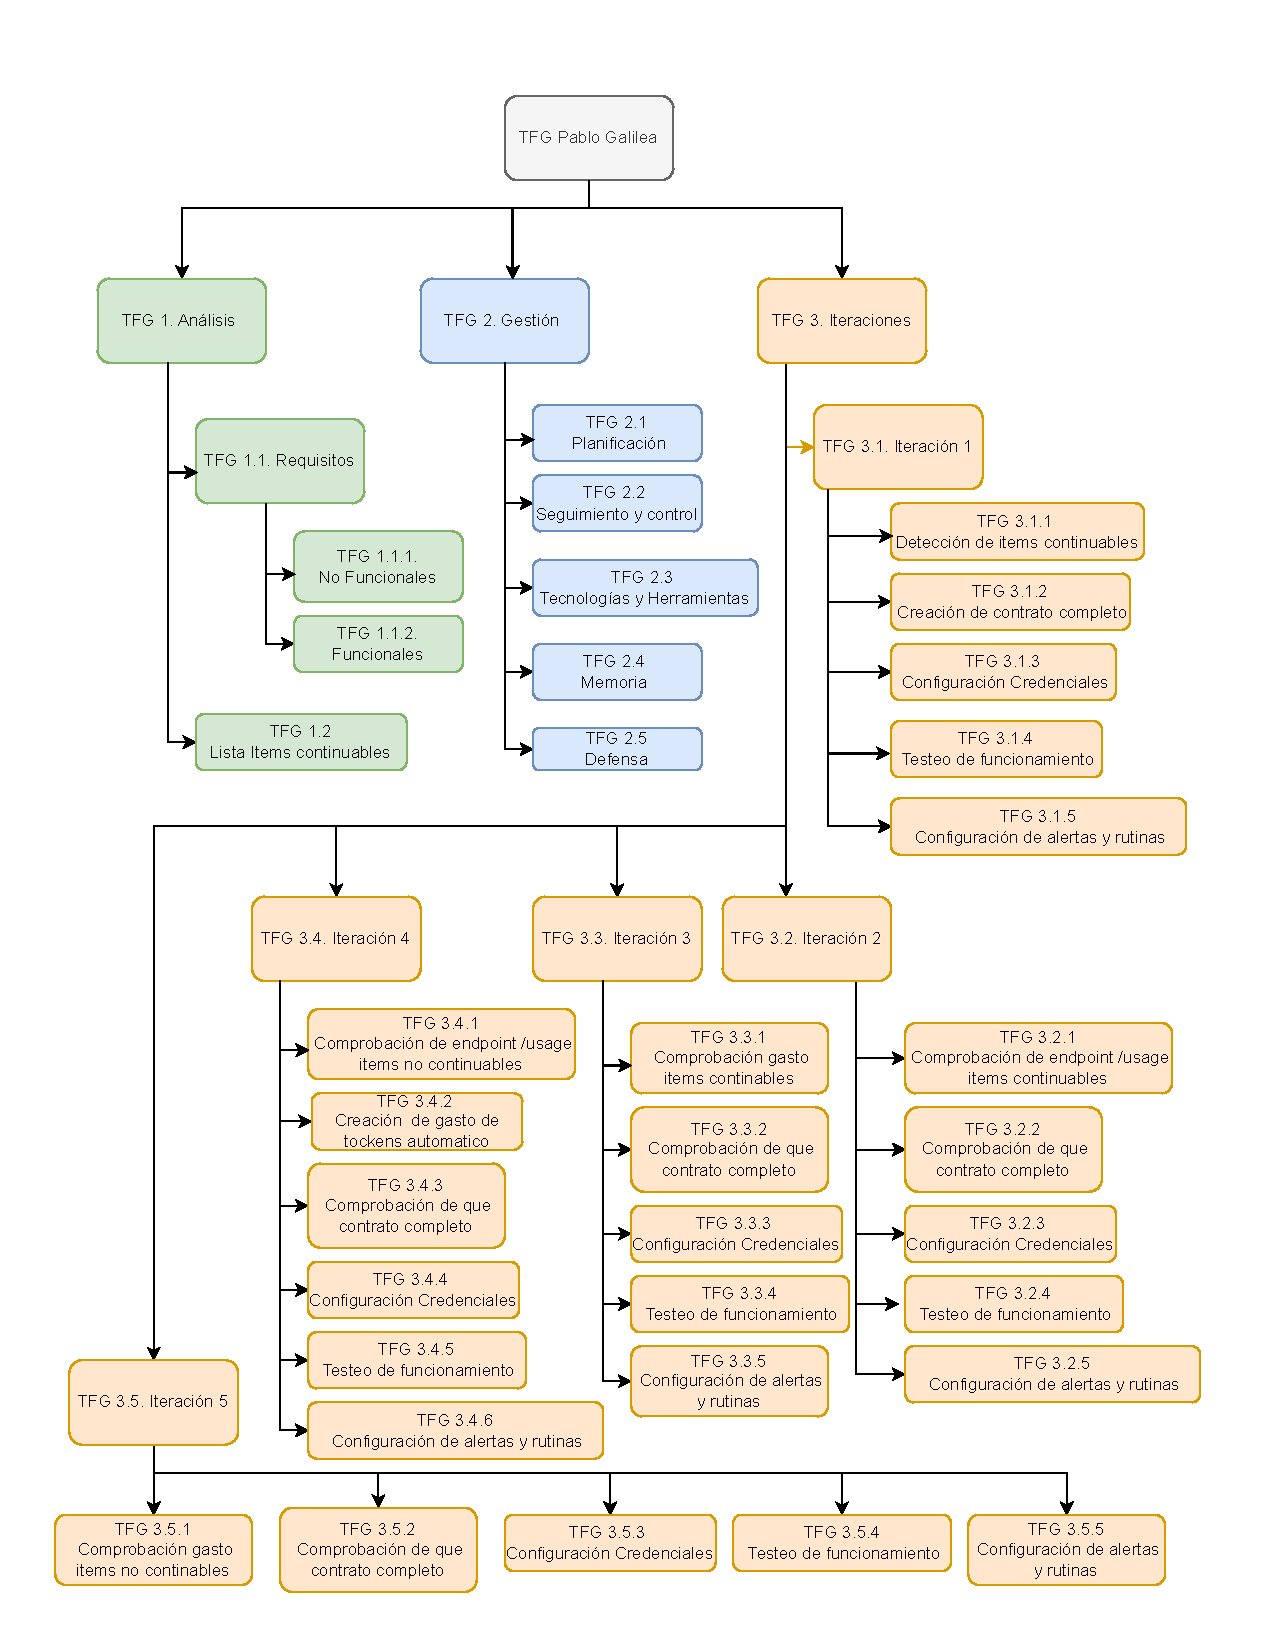
\includegraphics[width=0.6\textwidth]{archivos/EDT.pdf}
    \caption{EDT}
    \label{fig:edt}
\end{figure}
\subsection{Explicación del EDT}
En este apartado se describirán los diferentes módulos del EDT relacionandolos con los requisitos.
\begin{enumerate}
    % Configurar todos los niveles primero
    \renewcommand{\theenumii}{\theenumi.\arabic{enumii}}
    \renewcommand{\theenumiii}{\theenumii.\arabic{enumiii}}
    \renewcommand{\labelenumii}{\theenumii}
    \renewcommand{\labelenumiii}{\theenumiii}

    \item \textbf{Análisis}
          \begin{enumerate}
              \item \textbf{Análisis de Requisitos:} Identificación, documentación y validación de las necesidades del proyecto para definir las funcionalidades (funcionales) y restricciones (no funcionales) de un sistema.
                    \setcounter{enumiii}{0} % Reiniciar contador del tercer nivel
                    \begin{enumerate}
                        \item \textbf{No Funcionales:} Lista de aquellos requisitos que, aunque no añaden funcionalidad al proyecto, son importantes a tener en cuenta para lograr su ejecución.
                        \item \textbf{Funcionales:} Lista de aquellos requisitos necesarios para lograr que el proyecto cumpla con todas las características necesarias para que sea funcional.
                    \end{enumerate}
              \item \textbf{Lista de items continuables:} Lista con todos los SKUs de los recursos activos del DCD, omitiendo los obsoletos. Esta lista es necesaria para cumplir el requisito RF01.02 y permite identificar los elementos de mayor coste, información requerida para el requisito RF01.03 y RNF04.
          \end{enumerate}

    \item \textbf{Gestión}
          \setcounter{enumii}{0} % Reiniciar contador del segundo nivel
          \begin{enumerate}
              \item \textbf{Planificación: } Proceso de definir objetivos, tareas, recursos, costos y cronogramas para guiar la ejecución y asegurar el éxito, en el que se decide y especifica el cumplimiento de los requisitos RNF05 a RNF09.
              \item  \textbf{Seguimiento y Control: }Tras la implementación y la finalización del proyecto se hace un seguimiento de su correcto funcionamiento. Fundamental para lograr el requisito RNF01 y RNFO2.
              \item \textbf{Tecnologías y Herramientas: } Son las metodologías y enfoques que se han usado para la elaboración del proyecto y desarrollan los requisitos RNF05 a RNF09
              \item \textbf{Memoria:} El proceso de documentación del proyecto para poder analizarlo.
              \item \textbf{Defensa:} Argumentos y explicación sobre el proyecto para poder exponerlo a un tribunal ante posibles dudas.
          \end{enumerate}

    \item \textbf{Iteraciones}
          \setcounter{enumii}{0} % Reiniciar contador del segundo nivel
          \begin{enumerate}
              \item \textbf{Iteración 1:} Siendo esta la primera iteración, es en la que se crea la base en la que se basarán el resto de iteraciones, por lo que se deben tomar sus decisiones teniendo en cuenta que podrían afectar al resto del proceso. En esta primera iteración se detectarán los elementos que forman un contrato.
                    \setcounter{enumiii}{0} % Reiniciar contador del tercer nivel si es necesario
                    \begin{enumerate}
                        \item \textbf{Detección de items continuables:} La funcionalidad añadida en esta primera iteración se basa en lograr detectar qué SKUs forman parte de la lista creada. Como el contrato será creado por nosotros, se añadirán todos los SKUs, así que todos deberán estar; todo el que falte será un falso positivo.
                        \item \textbf{Creación de contrato completo:} De manera manual se crea un contrato con todos los SKUs de la lista. Cumpliendo asi el requisito RF01.01, RF02.01,RF02.01.01,RF02.01.02 y RF02.03.
                        \item \textbf{Configuración de Credenciales:} Esto se hace en todas las iteraciones, por lo que no se explicará en el resto, solo en esta. Se basa en la configuración concreta de CouchDB para el correcto funcionamiento. Cumpliendo así el requisito RF02.02.
                        \item \textbf{Testeo de funcionamiento: } Al igual que el anterior, este paso se hace en todas las iteraciones, por lo que solo se explicará en esta. En este apartado se crean las comprobaciones del correcto funcionamiento de esta y de las anteriores iteraciones.
                        \item \textbf{Configuración de alertas y rutinas: } Este apartado tiene la misma peculiaridad que los otros dos anteriores, por lo que se explicará solo en esta ocasión y se basa en crear las alertas que se enviarán en caso de fallo dependiendo de la información que ya se disponga, en este caso los SKUs que faltan y también crear el disparador para que se ejecute en cierto momento.

                    \end{enumerate}


              \item \textbf{Iteración 2:} En esta iteración ya se implementa el medir el uso de los SKUs continuables detectados en la iteración anterior y compararla con la esperada.
                    \setcounter{enumiii}{0} % Reiniciar contador del tercer nivel si es necesario
                    \begin{enumerate}
                        \item \textbf{Detección de endpoint /usage items continuables: } Para comprobar el uso de los elementos del DCD por medio de su API se puede comprobar con /usage.
                        \item \textbf{Comprobación de que contrato completo:} Se comprueba que no haya que añadir nada nuevo al contrato, en caso de ser necesario se añade y como será igual en el resto de iteraciones tampoco se añadirá.
                    \end{enumerate}


              \item \textbf{Iteración 3:} En esta iteración sabiendo el uso de los diferentes elementos se calcula su gasto económico teórico y se comprueba con el real.
                    \setcounter{enumiii}{0} % Reiniciar contador del tercer nivel si es necesario
                    \begin{enumerate}
                        \item \textbf{Comprobación gasto items continuables: } Sabiendo el gasto se calcula el precio de cada uno y se compara con el proporcionado por la API.
                    \end{enumerate}


              \item \textbf{Iteración 4:} En esta iteración se pasa a los items no continuables, por lo que se estudia cómo hacer un gasto relativamente constante de estos.
                    \setcounter{enumiii}{0} % Reiniciar contador del tercer nivel si es necesario
                    \begin{enumerate}
                        \item \textbf{Comprobación de endpoint /usage items no continuables: } Se comprueba el gasto de items no continuables por medio de su SKU.
                        \item \textbf{Creación de gasto de tokens automático:} Se estudia cómo lograr un gasto lo más constante posible de tokens.
                    \end{enumerate}


              \item \textbf{Iteración 5:} Teniendo ya el gasto, se calcula su precio y se comprueba con el gasto proporcionado por la API.
                    \setcounter{enumiii}{0} % Reiniciar contador del tercer nivel si es necesario
                    \begin{enumerate}
                        \item \textbf{Comprobación gasto items no continuables:} Se comprueba el gasto económico de items no continuables por medio de su SKU comparándolo con el obtenido en la API.
                    \end{enumerate}
          \end{enumerate}
\end{enumerate}
\newpage

\section{Estimación de tiempos}




\begin{table}[h!]
    \centering
    \small
    \begin{tabular}{|c|c|c|c|}
        \hline
        \multicolumn{4}{|c|}{Plan de dedicación de tiempo}                                                                       \\
        \hline
        Bloque                               & Nodo                                             & Tiempo & Total                 \\
        \hline
        \multirow{3}{*}{Análisis}            & Lista requisitos funcionales                     & 5h     & \multirow{3}{*}{15h}  \\
        \cline{2-3}
                                             & Análisis de requisitos Funcionales               & 5h     &                       \\
        \cline{2-3}
                                             & Análisis de requisitos no Funcionales            & 5h     &                       \\
        \hline
        \multirow{5}{*}{Gestión}             & Planificación                                    & 35h    & \multirow{5}{*}{141h} \\
        \cline{2-3}
        Cronograma de tareas                 & Seguimiento y control                            & 10h    &                       \\
        \cline{2-3}
                                             & Tecnologías y Herramientas                       & 6h     &                       \\
        \cline{2-3}
                                             & Memoria                                          & 75h    &                       \\
        \cline{2-3}
                                             & Defensa                                          & 15h    &                       \\
        \hline
        \multirow{5}{*}{Iteración 1}         & Detección de items continuables                  & 16h    & \multirow{5}{*}{42h}  \\
        \cline{2-3}
                                             & Creación de contrato completo                    & 12h    &                       \\
        \cline{2-3}
                                             & Configuración de credenciales                    & 6h     &                       \\
        \cline{2-3}
                                             & Testeo de funcionamiento                         & 4h     &                       \\
        \cline{2-3}
                                             & Configuración de alertas y rutinas               & 4h     &                       \\
        \hline
        \multirow{5}{*}{Iteración 2}         & Comprobación de /usage items continuables        & 16h    & \multirow{5}{*}{21h}  \\
        \cline{2-3}
                                             & Comprobación de que contrato completo            & 1h     &                       \\
        \cline{2-3}
                                             & Configuración de credenciales, alertas y rutinas & 2h     &                       \\
        \cline{2-3}
                                             & Testeo de funcionamiento                         & 2h     &                       \\
        \hline
        \multirow{5}{*}{Iteración 3}         & Comprobación gasto items continuables            & 16h    & \multirow{5}{*}{23h}  \\
        \cline{2-3}
                                             & Comprobación de que contrato completo            & 1h     &                       \\
        \cline{2-3}
                                             & Configuración de credenciales ,alertas y rutinas & 2h     &                       \\
        \cline{2-3}
                                             & Testeo de funcionamiento                         & 4h     &                       \\
        \hline
        \multirow{6}{*}{Iteración 4}         & Comprobación de /usage items no continuables     & 12h    & \multirow{6}{*}{37h}  \\
        \cline{2-3}
                                             & Creación de gasto de tokens automático           & 16h    &                       \\
        \cline{2-3}
                                             & Comprobación de que contrato completo            & 1h     &                       \\
        \cline{2-3}
                                             & Configuración de credenciales, alertas y rutinas & 4h     &                       \\
        \cline{2-3}
                                             & Testeo de funcionamiento                         & 4h     &                       \\
        \hline
        \multirow{5}{*}{Iteración 5}         & Comprobación gasto items no continuables         & 10h    & \multirow{5}{*}{21h}  \\
        \cline{2-3}
                                             & Comprobación de que contrato completo            & 1h     &                       \\
        \cline{2-3}
                                             & Configuración de credenciales, alertas y rutinas & 4h     &                       \\
        \cline{2-3}
                                             & Testeo de funcionamiento                         & 6h     &                       \\
        \hline
        \multicolumn{2}{|c|}{Total de Horas} & \multicolumn{2}{|c|}{300 h}                                                       \\
        \hline
    \end{tabular}
    \caption{Plan de dedicación de tiempos}
\end{table}

\section{Cronograma e hitos}

% Definir colores
\definecolor{ganttblue}{RGB}{173,216,230}
\definecolor{ganttgreen}{RGB}{144,238,144}



\begin{table}[h!]
    \centering
    \footnotesize
    \setlength{\tabcolsep}{3pt}
    \begin{tabular}{|c|l|c|c|c|c|c|c|c|c|c|c|c|c|} % <- segunda columna: l
        \hline
        \multicolumn{14}{|c|}{\textbf{Cronograma de tareas}}                                                                                                                                                                                                                                                                                                                  \\
        \hline
        \multicolumn{2}{|c|}{\multirow{2}{*}{\textbf{Paquete de trabajo}}}
                               & \multicolumn{4}{|c|}{\textbf{Febrero}}
                               & \multicolumn{4}{|c|}{\textbf{Marzo}}
                               & \multicolumn{4}{|c|}{\textbf{Abril}}                                                                                                                                                                                                                                                                                                         \\
        \cline{3-14}
        \multicolumn{2}{|c|}{} & S1                                           & S2                    & S3                    & S4                    & S5                    & S6                    & S7                    & S8                    & S9                    & S10                   & S11                   & S12                                           \\
        \hline
        TFG 1.1.1              & Análisis de requisitos no funcionales        & \cellcolor{ganttblue} & \cellcolor{ganttblue} &                       &                       &                       &                       &                       &                       &                       &                       &                       & \hspace{0pt}          \\ % <- truco para la última columna
        \hline
        TFG 1.1.2              & Análisis de requisitos funcionales           & \cellcolor{ganttblue} & \cellcolor{ganttblue} &                       &                       &                       &                       &                       &                       &                       &                       &                       & \hspace{0pt}          \\
        \hline
        TFG 1.2                & Lista Items continuables                     &                       & \cellcolor{ganttblue} &                       &                       &                       &                       &                       &                       &                       &                       &                       & \hspace{0pt}          \\
        \hline
        TFG 2.1                & Planificación                                & \cellcolor{ganttblue} & \cellcolor{ganttblue} & \cellcolor{ganttblue} & \cellcolor{ganttblue} & \cellcolor{ganttblue} &                       &                       &                       &                       &                       &                       & \hspace{0pt}          \\
        \hline
        TFG 2.2                & Seguimiento y control                        &                       &                       &                       &                       &                       & \cellcolor{ganttblue} & \cellcolor{ganttblue} & \cellcolor{ganttblue} & \cellcolor{ganttblue} & \cellcolor{ganttblue} & \cellcolor{ganttblue} & \cellcolor{ganttblue} \\
        \hline
        TFG 2.3                & Tecnologías y herramientas                   &                       &                       &                       & \cellcolor{ganttblue} & \cellcolor{ganttblue} &                       &                       &                       &                       &                       &                       & \hspace{0pt}          \\
        \hline
        TFG 2.4                & Memoria                                      &                       &                       &                       & \cellcolor{ganttblue} & \cellcolor{ganttblue} & \cellcolor{ganttblue} & \cellcolor{ganttblue} & \cellcolor{ganttblue} & \cellcolor{ganttblue} & \cellcolor{ganttblue} & \cellcolor{ganttblue} & \cellcolor{ganttblue} \\
        \hline
        TFG 3.1.1              & Detección de items continuables              &                       &                       &                       & \cellcolor{ganttblue} & \cellcolor{ganttblue} &                       &                       &                       &                       &                       &                       & \hspace{0pt}          \\
        \hline
        TFG 3.1.2              & Creación de contrato completo                &                       & \cellcolor{ganttblue} & \cellcolor{ganttblue} & \cellcolor{ganttblue} &                       &                       &                       &                       &                       &                       &                       & \hspace{0pt}          \\
        \hline
        TFG 3.x.3              & Configuración Credenciales                   &                       &                       & \cellcolor{ganttblue} & \cellcolor{ganttblue} & \cellcolor{ganttblue} & \cellcolor{ganttblue} & \cellcolor{ganttblue} & \cellcolor{ganttblue} & \cellcolor{ganttblue} & \cellcolor{ganttblue} & \cellcolor{ganttblue} & \cellcolor{ganttblue} \\
        \hline
        TFG 3.x.4              & Testeo funcionamiento                        &                       &                       &                       &                       & \cellcolor{ganttblue} & \cellcolor{ganttblue} & \cellcolor{ganttblue} & \cellcolor{ganttblue} & \cellcolor{ganttblue} & \cellcolor{ganttblue} & \cellcolor{ganttblue} & \cellcolor{ganttblue} \\
        \hline
        TFG 3.x.5              & Configuración de alertas y rutinas           &                       &                       &                       &                       & \cellcolor{ganttblue} & \cellcolor{ganttblue} & \cellcolor{ganttblue} & \cellcolor{ganttblue} & \cellcolor{ganttblue} & \cellcolor{ganttblue} & \cellcolor{ganttblue} & \cellcolor{ganttblue} \\
        \hline
        TFG 3.2.1              & Comprobación de /usage items continuable     &                       &                       &                       &                       &                       & \cellcolor{ganttblue} & \cellcolor{ganttblue} &                       &                       &                       &                       & \hspace{0pt}          \\
        \hline
        TFG 3.x.2              & Comprobación de que contrato completo        &                       &                       &                       &                       &                       & \cellcolor{ganttblue} & \cellcolor{ganttblue} & \cellcolor{ganttblue} & \cellcolor{ganttblue} & \cellcolor{ganttblue} & \cellcolor{ganttblue} & \cellcolor{ganttblue} \\
        \hline
        TFG 3.3.1              & Comprobación gasto items continuables        &                       &                       &                       &                       &                       &                       &                       & \cellcolor{ganttblue} & \cellcolor{ganttblue} &                       &                       & \hspace{0pt}          \\
        \hline
        TFG 3.4.1              & Comprobación de /usage items no continuables &                       &                       &                       &                       &                       &                       &                       &                       &                       & \cellcolor{ganttblue} & \cellcolor{ganttblue} & \hspace{0pt}          \\
        \hline
        TFG 3.4.2              & Creación de gasto de tokens automático       &                       &                       &                       &                       &                       &                       &                       &                       & \cellcolor{ganttblue} & \cellcolor{ganttblue} &                       &                       \\
        \hline
        TFG 3.5.1              & Comprobación gasto items no continuables     &                       &                       &                       &                       &                       &                       &                       &                       &                       &                       &                       & \cellcolor{ganttblue} \\
        \hline
    \end{tabular}
    \caption{Cronograma de tareas del TFG}
\end{table}

\begin{table}[h!]
    \centering
    \footnotesize
    \setlength{\tabcolsep}{3pt}
    \begin{tabular}{|c|l|c|c|c|c|c|c|c|c|c|c|c|c|}
        \hline
        \multicolumn{14}{|c|}{\textbf{Cronograma de tareas II}}                                                                                                                                                                                                                                                                                   \\
        \hline
        \multicolumn{2}{|c|}{\multirow{2}{*}{\textbf{Paquete de trabajo}}}
                               & \multicolumn{4}{|c|}{\textbf{Mayo}}
                               & \multicolumn{4}{|c|}{\textbf{Junio}}
                               & \multicolumn{4}{|c|}{\textbf{Julio}}                                                                                                                                                                                                                                                                             \\
        \cline{3-14}
        \multicolumn{2}{|c|}{} & S13                                      & S14                   & S15                                        & S16                   & S17                   & S18                   & S19                   & S20                   & S21                   & S22                   & S23 & S24                \\
        \hline

        TFG 2.2                & Seguimiento y control                    & \cellcolor{ganttblue} & \cellcolor{ganttblue}                      & \cellcolor{ganttblue} & \cellcolor{ganttblue} & \cellcolor{ganttblue} & \cellcolor{ganttblue} &                       &                       &                       &     &     & \hspace{0pt} \\
        \hline
        TFG 2.4                & Memoria                                  & \cellcolor{ganttblue} & \cellcolor{ganttblue}                      & \cellcolor{ganttblue} & \cellcolor{ganttblue} & \cellcolor{ganttblue} & \cellcolor{ganttblue} & \cellcolor{ganttblue} &                       &                       &     &     & \hspace{0pt} \\
        \hline
        TFG 2.4                & Defensa                                  &                       &                                            &                       &                       &                       &                       &                       & \cellcolor{ganttblue} & \cellcolor{ganttblue} &     &     & \hspace{0pt} \\
        \hline
        TFG 3.x.4              & Testeo funcionamiento                    & \cellcolor{ganttblue} & \cellcolor{ganttblue}                      & \cellcolor{ganttblue} &                       &                       &                       &                       &                       &                       &     &     & \hspace{0pt} \\
        \hline
        TFG 3.x.5              & Configuración de alertas y rutinas       & \cellcolor{ganttblue} & \cellcolor{ganttblue}\cellcolor{ganttblue} &                       &                       &                       &                       &                       &                       &                       &     &     & \hspace{0pt} \\
        \hline
        TFG 3.5.1              & Comprobación gasto items no continuables & \cellcolor{ganttblue} & \cellcolor{ganttblue}                      &                       &                       &                       &                       &                       &                       &                       &     &     & \hspace{0pt} \\
        \hline
    \end{tabular}
    \caption{Cronograma de tareas del TFG}
\end{table}

Sabiendo ya el cronograma se pueden marcar la fecha de finalización de los distintos hitos.
\begin{table}[
    ]
    \centering
    \begin{tabular}{|c|l|l|}
        \hline
        \multicolumn{2}{|c|}{\textbf{Hitos} } & \textbf{Fecha finalización}                                          \\
        \hline
        TFG 1.1.1                             & Análisis de requisitos no funcionales        & 12 de febrero de 2026 \\
        \hline
        TFG 1.1.2                             & Análisis de requisitos funcionales           & 13 de febrero de 2026 \\
        \hline
        TFG 1.2                               & Lista Items continuables                     & 14 de febrero de 2026 \\
        \hline
        TFG 2.1                               & Planificación                                & 5 de marzo de 2026    \\
        \hline
        TFG 2.2                               & Seguimiento y control                        & 15 de junio de 2026   \\
        \hline
        TFG 2.3                               & Tecnologías y herramientas                   & 7 de marzo de 2026    \\
        \hline
        TFG 2.4                               & Memoria                                      & 22 de junio de 2026   \\
        \hline
        TFG 2.5                               & Defensa                                      & 3 de julio de 2026    \\
        \hline
        TFG 3.1.1                             & Detección de items continuables              & 7 de marzo de 2026    \\
        \hline
        TFG 3.1.2                             & Creación de contrato completo                & 28 de febrero de 2026 \\
        \hline
        TFG 3.1.3                             & Configuración Credenciales (1)               & 5 de marzo de 2026    \\
        \hline
        TFG 3.1.4                             & Testeo funcionamiento (1)                    & 12 de marzo de 2026   \\
        \hline
        TFG 3.1.5                             & Configuración de alertas y rutinas (1)       & 11 de marzo de 2026   \\
        \hline
        TFG 3.2.1                             & Comprobación de /usage items continuable     & 25 de marzo de 2026   \\
        \hline
        TFG 3.2.2                             & Comprobación de que contrato completo (2)    & 14 de marzo de 2026   \\
        \hline
        TFG 3.2.3                             & Configuración Credenciales(2)                & 20 de marzo de 2026   \\
        \hline
        TFG 3.3.4                             & Testeo funcionamiento (2)                    & 29 de marzo de 2026   \\
        \hline
        TFG 3.4.5                             & Configuración de alertas y rutinas (2)       & 27 de marzo de 2026   \\
        \hline
        TFG 3.3.1                             & Comprobación gasto items continuables        & 3 de abril de 2026    \\
        \hline
        TFG 3.3.2                             & Comprobación de que contrato completo (3)    & 29 de marzo de 2026   \\
        \hline
        TFG 3.3.3                             & Configuración Credenciales (3)               & 1 de abril de 2026    \\
        \hline
        TFG 3.3.4                             & Testeo funcionamiento (3)                    & 5 de abril de 2026    \\
        \hline
        TFG 3.3.5                             & Configuración de alertas y rutinas (3)       & 6 de abril de 2026    \\
        \hline
        TFG 3.4.1                             & Comprobación de /usage items no continuables & 23 de abril de 2026   \\
        \hline
        TFG 3.4.2                             & Creación de gasto de tokens automático       & 20 de abril de 2026   \\
        \hline
        TFG 3.4.3                             & Comprobación de que contrato completo (4)    & 16 de abril de 2026   \\
        \hline
        TFG 3.4.4                             & Configuración Credenciales (4)               & 17 de abril de 2026   \\
        \hline
        TFG 3.4.5                             & Testeo funcionamiento (4)                    & 24 de abril de 2026   \\
        \hline
        TFG 3.4.6                             & Configuración de alertas y rutinas (4)       & 25 de abril de 2026   \\
        \hline
        TFG 3.5.1                             & Comprobación gasto items no continuables     & 7 de mayo de 2026     \\
        \hline
        TFG 3.5.2                             & Comprobación de que contrato completo (5)    & 23 de abril de 2026   \\
        \hline
        TFG 3.5.3                             & Configuración Credenciales (5)               & 24 de abril de 2026   \\
        \hline
        TFG 3.5.4                             & Testeo funcionamiento (5)                    & 9 de mayo de 2026     \\
        \hline
        TFG 3.5.5                             & Configuración de alertas y rutinas (5)       & 11 de mayo de 2026    \\
        \hline
    \end{tabular}
    \caption{Hitos TFG}
    \label{tab:placeholder}
\end{table}
\section{Plan de contingencias y riesgos}
Siendo un proyecto de cierto tamaño, hay muchos factores que se pueden no tener en cuenta, debido a que cuanto más grande sea un proyecto más posibles problemas pueden ocurrir, por lo que para poder minimizar esos riesgos, se crea un plan de contingencia ante posibles riesgos, para proteger los activos más valiosos. Para hacerlo, se basará en el análisis de riesgos estudiado en la asignatura de Seguridad de esta titulación, impartida en esta universidad.
\begin{table}[h!]
    \centering
    \small
    \begin{tabular}{|p{1.5cm}|p{2cm}|p{2cm}|p{1.5cm}|p{3.8cm}|p{1.8cm}|}
        \hline
        \multicolumn{6}{|c|}{\textbf{Plan de contingencias y riesgos}}                                                                                                                                                                                                                                                                                                                                                                                                                                   \\
        \hline
        \textbf{Origen} & \textbf{Riesgo}                                                                                                                                                              & \textbf{Probabilidad} & \textbf{Impacto} & \textbf{Solución}                                                                                                                                                                                                          & \textbf{Tipo de medida} \\
        \hline
        Hardware        & Destrucción o pérdida del ordenador de trabajo                                                                                                                               & baja                  & alto             & Para evitar la pérdida de toda la información se hará una estrategia 2+1: dos copias en la nube con guardado de versiones (GitHub y GitLab) y una copia de seguridad periódica en un disco físico guardado y desconectado. & Preventiva              \\
        \hline
        Humano          & Siendo una sola persona la que participa en el proyecto, es posible que se encuentre indispuesto por diversas causas como enfermedad, por lo que se paralizaría el proyecto. & Media                 & Medio            & Dejar espacio suficiente entre la finalización teórica del proyecto y la entrega real, para poder compensar posibles ausencias.                                                                                            & Preventiva              \\
        \hline
    \end{tabular}
    \caption{Plan de contingencias y riesgos}
\end{table}


\begin{table}[h!]
    \centering
    \small
    \begin{tabular}{|p{1.5cm}|p{2cm}|p{2cm}|p{1.5cm}|p{3.8cm}|p{1.8cm}|}
        \hline
        \multicolumn{6}{|c|}{\textbf{Plan de contingencias y riesgos}}                                                                                                                                                                                                                                                                                                                                    \\
        \hline
        \textbf{Origen} & \textbf{Riesgo}                                                                                                                          & \textbf{Probabilidad} & \textbf{Impacto} & \textbf{Solución}                                                                                                                                               & \textbf{Tipo de medida} \\
        \hline
        Datos           & Trabajando con recursos valiosos puede haber intentos de robo de información, como contraseñas o tokens de APIs privadas de IONOS Cloud. & Media                 & Alto             & Almacenamiento de estas credenciales en entornos seguros como KeePassXC y no incluirlas en el código.                                                           & Preventiva              \\
        \hline
        Software        & Cambios en las APIs usadas                                                                                                               & Bajo                  & Alto             & Usar versiones estables de las APIs y controlar posibles cambios para mantener el uso de las APIs antiguas o, en caso de estar obsoletas, cambiar a las nuevas. & Preventiva              \\
        \hline
    \end{tabular}
    \caption{Plan de contingencias y riesgos}
\end{table}

\clearpage

\subsection{Flujo de Trabajo Canary}

\begin{figure}[h!]
    \centering
    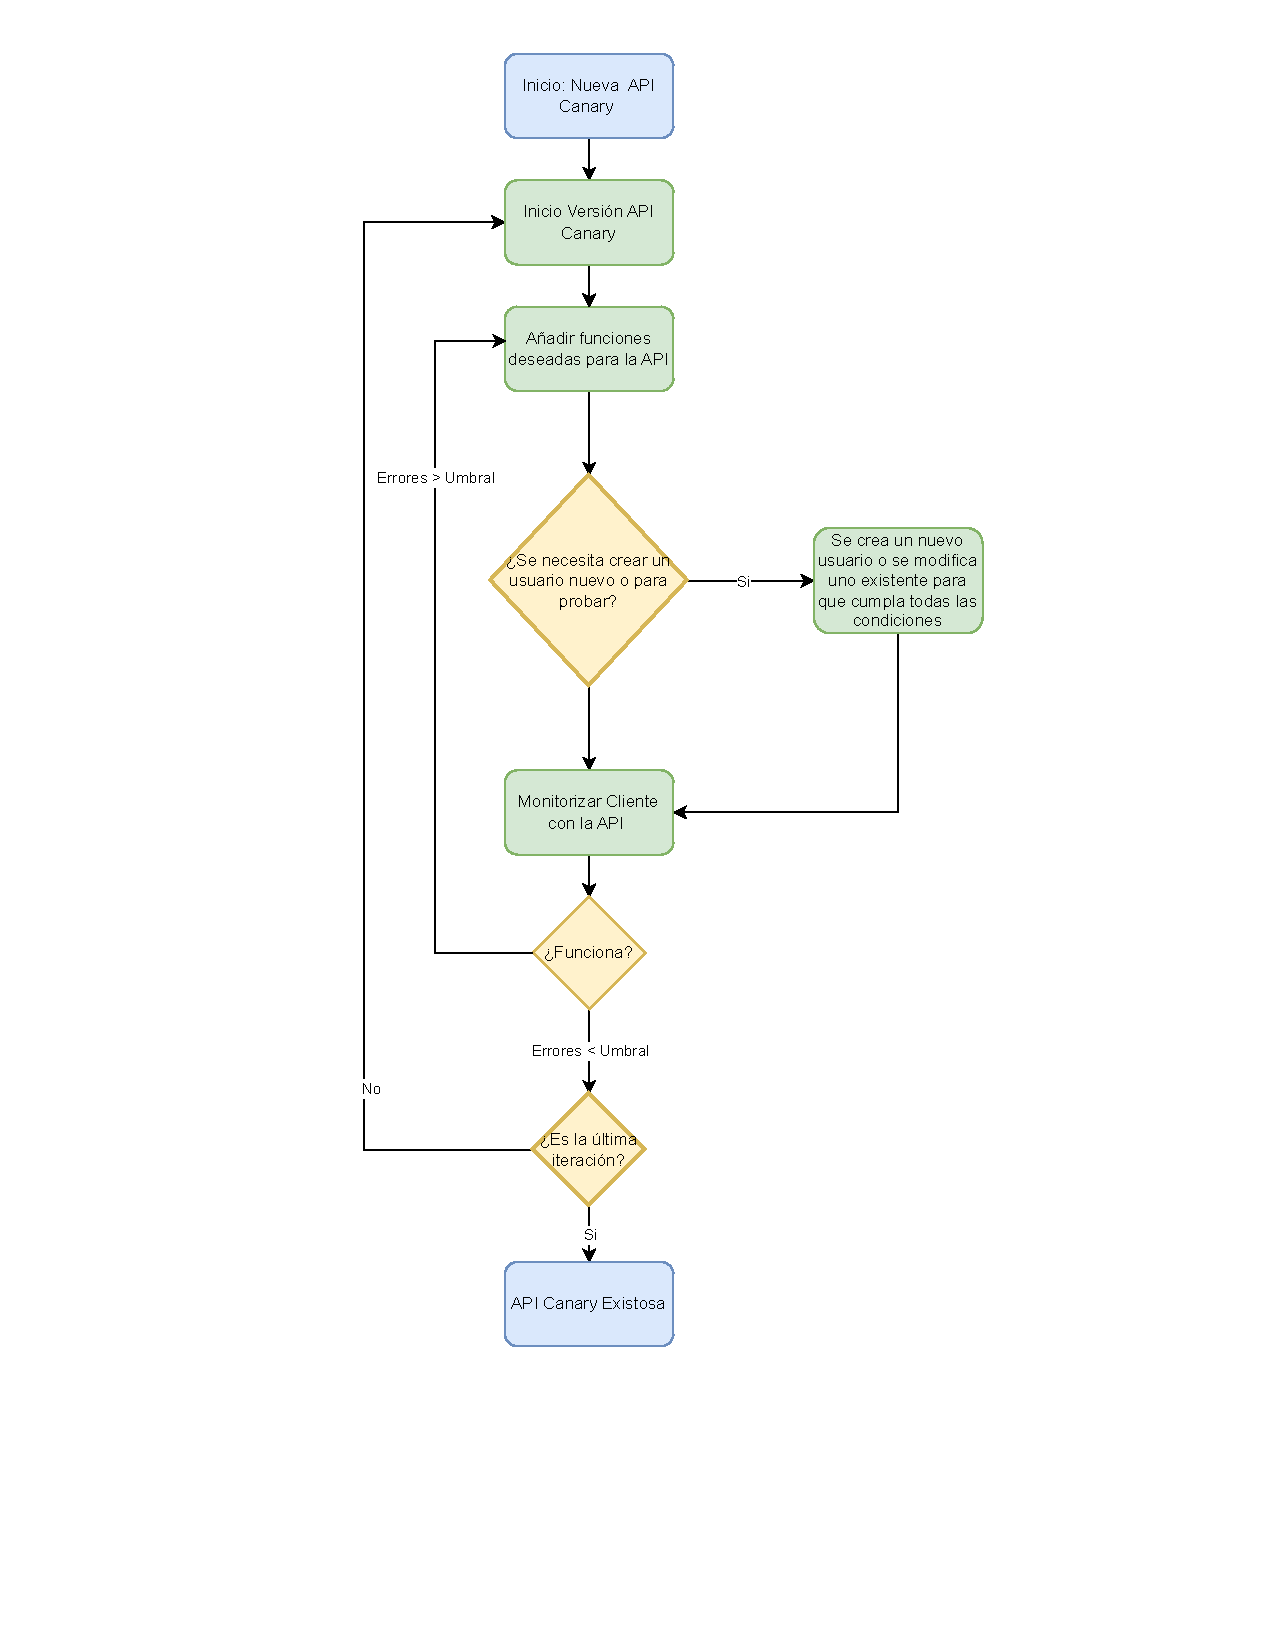
\includegraphics[width=0.9\textwidth]{archivos/flujo_API_Canary.drawio.pdf}
    \caption{Diagrama de flujo del proceso de despliegue Canary para APIs}
    \label{fig:canary-flow}
\end{figure}

\textbf{Descripción del flujo:}
\begin{enumerate}
    \item \textbf{Inicio: Nueva API Canary} - Desarrollo de una nueva API de validación.

    \item \textbf{Inicio: Nueva Versión API Canary} - Desarrollo de una nueva versión de la API de validación, en la que se inicia la nueva iteración.

    \item \textbf{Inicio: Añadir funciones deseadas} - Se implementan las nuevas funciones deseadas.

    \item \textbf{Comprobación de completitud del usuario de muestra} - Se comprueba que el usuario que se usa para comprobar el correcto funcionamiento de la API tiene todos los recursos necesarios que debe comprobar. En el caso contrario, se modifica para que permita comprobar todas las funciones a comprobar, en su defecto se creará un nuevo perfil para ello.

    \item \textbf{Monitorizar Métricas} - Análisis continuo de errores, latencia y otras métricas clave.

    \item \textbf{Decisión basada en umbrales:}
          \begin{itemize}
              \item \textbf{Si errores < Umbral} → Se pasa a la siguiente fase de la API.
              \item \textbf{Si errores > Umbral} → Rollback automático a versión estable y se revisan las actualizaciones para volver a modificar y lograr hacer funcionales los cambios.
          \end{itemize}

    \item \textbf{API Canary Exitosa} - Tras terminar todas las fases, se integra y entra la fase de automatizarla para que se ejecute periódicamente.
\end{enumerate}



% ===== SECCIÓN 1.4: TECNOLOGIAS Y HERRAMIENTAS =====

\section{Tecnologías y Herramientas Utilizadas}

\noindent Para el desarrollo del sistema de validación de facturación cloud, se ha construido una arquitectura tecnológica robusta que combina herramientas modernas de desarrollo, infraestructura contenerizada y patrones de diseño específicos para el dominio de facturación.

\subsubsection{Stack Tecnológico Principal}

\begin{table}[h!]
    \centering
    \begin{tabular}{|p{0.25\textwidth}|p{0.7\textwidth}|}
        \hline
        \textbf{Categoría}                         & \textbf{Tecnologías}                    \\
        \hline
        \hline
        \textbf{Runtime}                           & Node.js 18+ (LTS)                       \\
        \hline
        \textbf{Lenguaje}                          & JavaScript ES6+ con módulos             \\
        \hline
        \textbf{Framework Web}                     & Express.js con middleware personalizado \\
        \hline
        \textbf{Gestión de Paquetes}               & Yarn 3+ con workspace                   \\
        \hline
        \textbf{Testing}                           & Postman                                 \\
        \hline
        \textbf{Creación de usuarios de muestreo } & DCD de IONOS                            \\
        \hline
        \textbf{Base de Datos Configuración}       & CouchDB para configuración distribuida  \\
        \hline
        \textbf{Control de Versiones}              & GitLab para paquetes internos           \\
        \hline
        \textbf{Editor de Código}                  & Visual Studio Code                      \\
        \hline
        \textbf{Documentación}                     & LaTeX en OverLeaf                       \\
        \hline
        \textbf{Creación de diagramas}             & Draw.io                                 \\
        \hline
        \textbf{Conexión con equipo }              & VPN a red Alemana                       \\
    \end{tabular}
    \caption{Stack tecnológico del proyecto}
    \label{tab:stack-tecnologico}
\end{table}

\subsubsection{Dependencias Clave del Proyecto}

\textbf{Dependencias Internas:}
\begin{itemize}
    \item \texttt{@internal/core} - Framework base con utilidades de inicialización y configuración
    \item \texttt{@internal/dev} - Suite de herramientas para desarrollo y debugging
\end{itemize}

\textbf{Dependencias Externas Críticas:}
\begin{itemize}
    \item \texttt{helmet} - Middleware de seguridad para cabeceras HTTP
    \item \texttt{express} - Framework web minimalista para Node.js
    \item \texttt{couchdb-nano} - Cliente para integración con CouchDB
\end{itemize}

\subsubsection{Arquitectura Modular Implementada}

La arquitectura del sistema se organiza en tres capas principales:

\begin{enumerate}
    \item \textbf{Capa de Infraestructura:}
          \begin{itemize}
              \item CouchDB para gestión de configuración centralizada
          \end{itemize}

    \item \textbf{Capa de Servicios:}
          \begin{itemize}
              \item \texttt{data-api}: Servicio de acceso y transformación de datos
              \item \texttt{invoice-validation}: Motor de validación de facturación
              \item \texttt{utilization}: Procesamiento de métricas de uso
          \end{itemize}

    \item \textbf{Capa de Helpers y Utilidades:}
          \begin{itemize}
              \item Módulo \texttt{schema}: Validación y transformación de datos
              \item Módulo \texttt{actions}: Operaciones comunes del negocio
              \item Módulo \texttt{invoice}: Lógica específica de facturación
          \end{itemize}
\end{enumerate}

\subsubsection{Flujo de Desarrollo y Calidad}

\begin{itemize}
    \item \textbf{Desarrollo Local:} Nodemon para hot-reload durante el desarrollo
    \item \textbf{Calidad de Código:} ESLint con configuración personalizada
    \item \textbf{Control de Cambios:} Hooks pre-commit para validaciones automáticas
    \item \textbf{Integración:} Pipelines CI/CD en GitLab para despliegue continuo
\end{itemize}


